\begin{figure}[htpb!]
\centering
\begin{subfigure}{.5\textwidth}
  \centering
  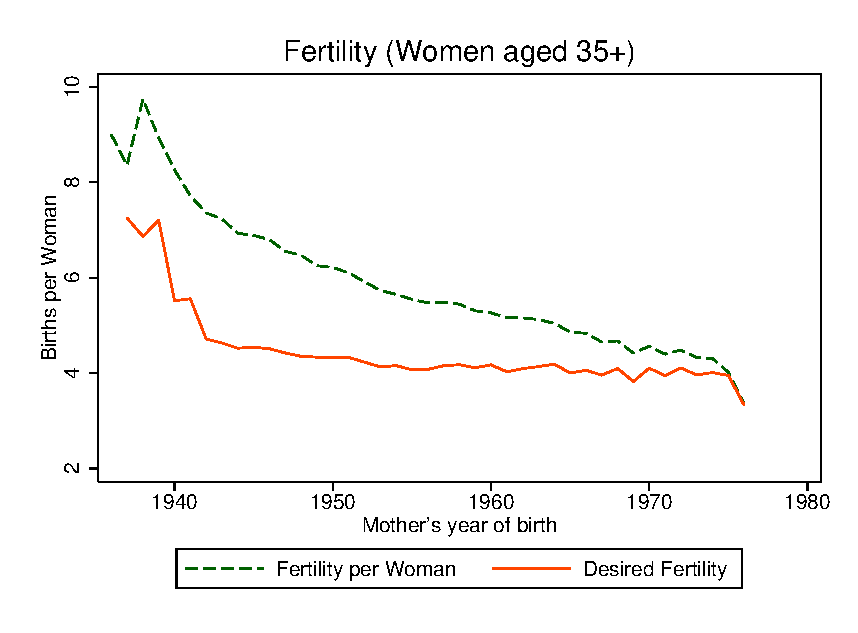
\includegraphics[scale=0.53]{\twinfolder/Figures/ferttrend_35_all.eps}
  \caption{Trends in Fertility}
  \label{TWINfig:fertrend}
\end{subfigure}%
\begin{subfigure}{.5\textwidth}
  \centering
  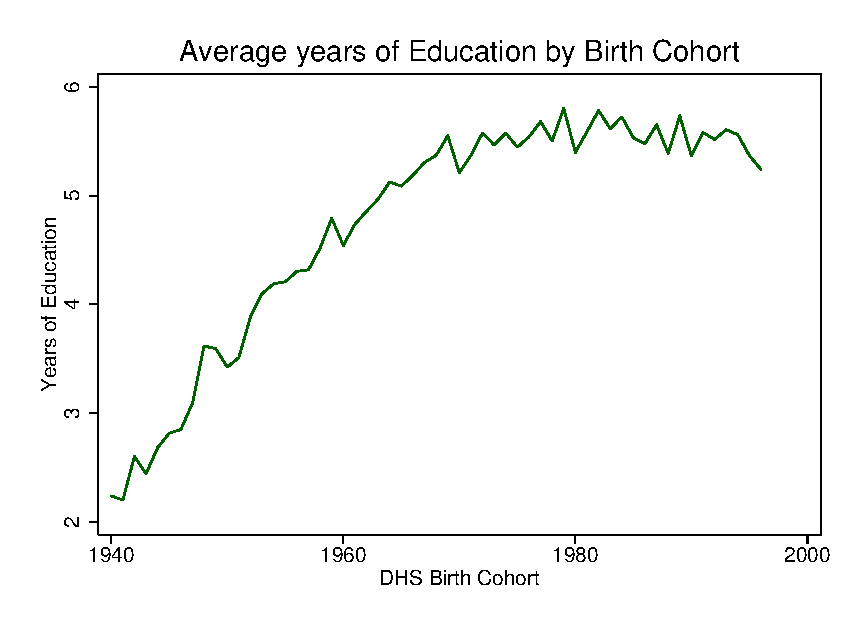
\includegraphics[scale=0.52]{\twinfolder/Figures/eductrend_all.eps}
  \caption{Trend in Education}
  \label{TWINfig:eductrend}
\end{subfigure}
\caption{Education and Fertility}
\label{TWINfig:trends}
\floatfoot{Note to figure \ref{TWINfig:trends}: Cohorts are made up of all individuals 
from the DHS who are over 35 years (for fertility), and over 15 years (for education).  
In each case the sample is restricted to those who have approximately completed fertility 
and education respectively.}
\end{figure}
\vspace{1cm}

\begin{figure}[htpb!]
\begin{center}
\caption{Proportion of Twins by Birth Order}
\label{TWINfig:bord}
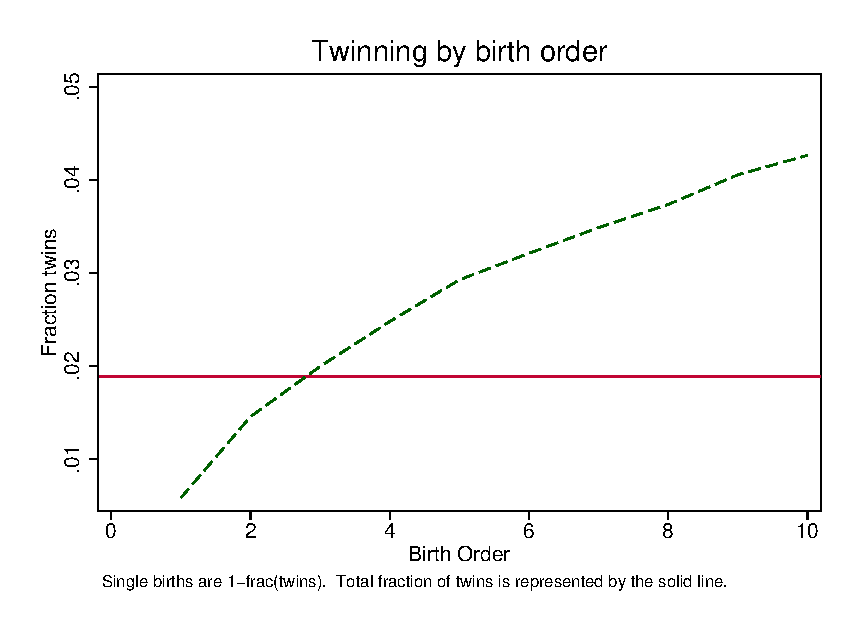
\includegraphics[scale=0.92]{\twinfolder/Figures/twinbybord.eps} 
\end{center}
\end{figure}

\begin{figure}[htpb!]
\begin{center}
\caption{Twin Births and Total Fertility}
\label{TWINfig:births}
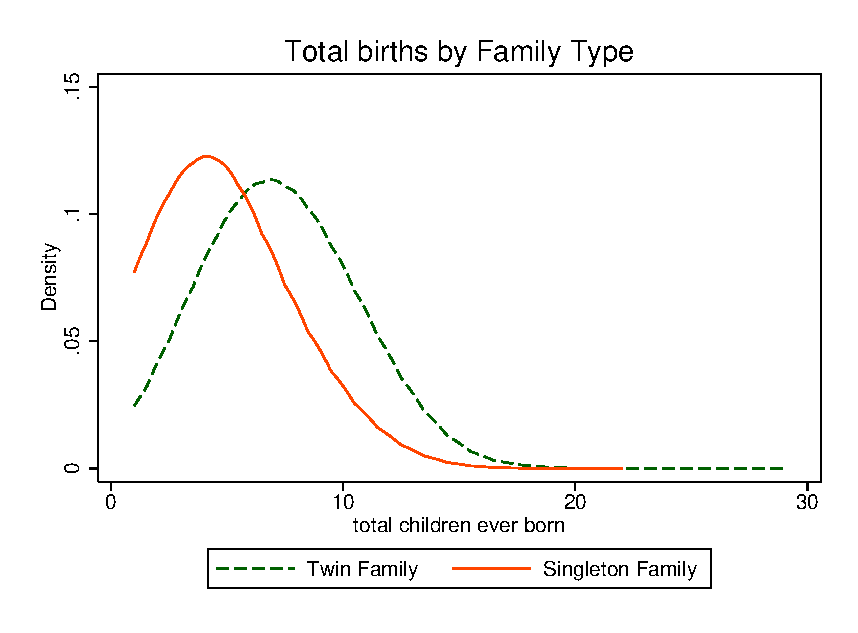
\includegraphics[scale=0.92]{\twinfolder/Figures/famsize.eps} 
\end{center}
\end{figure}

\begin{figure}[htpb!]
\begin{center}
\caption{Distribution of Ideal Family Size}
\label{TWINfig:ideal}
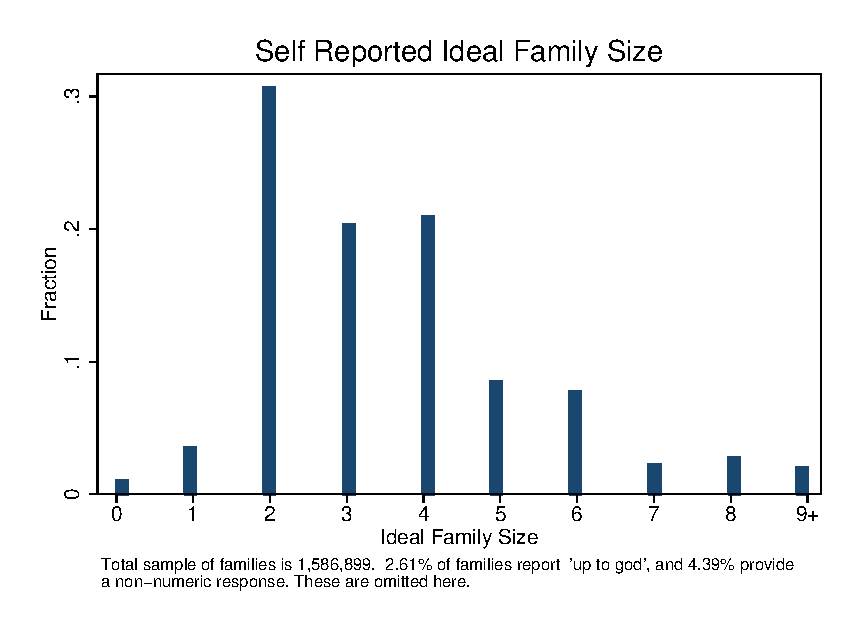
\includegraphics[scale=0.92]{\twinfolder/Figures/idealfamsize.eps} 
\end{center}
\end{figure}

\begin{figure}[htpb!]
\begin{center}
\caption{Ideal and Actual Fertility}
\label{TWINfig:idealactual}
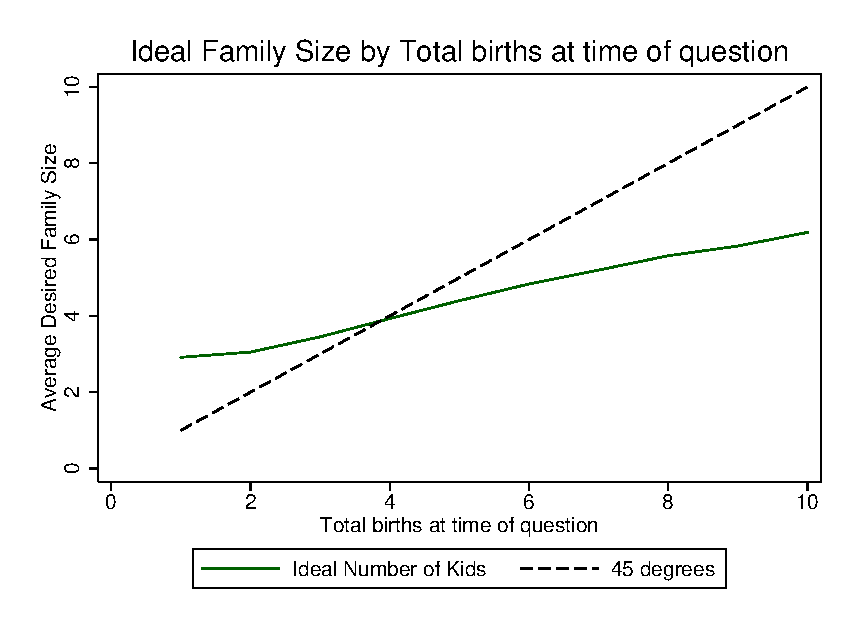
\includegraphics[scale=0.92]{\twinfolder/Figures/idealfam_fert.eps} 
\end{center}
\end{figure}

\begin{figure}[htpb!]
\begin{center}
\caption{Relaxing Strict Exogeneity (two plus)}
\label{TWINfig:ltz2}
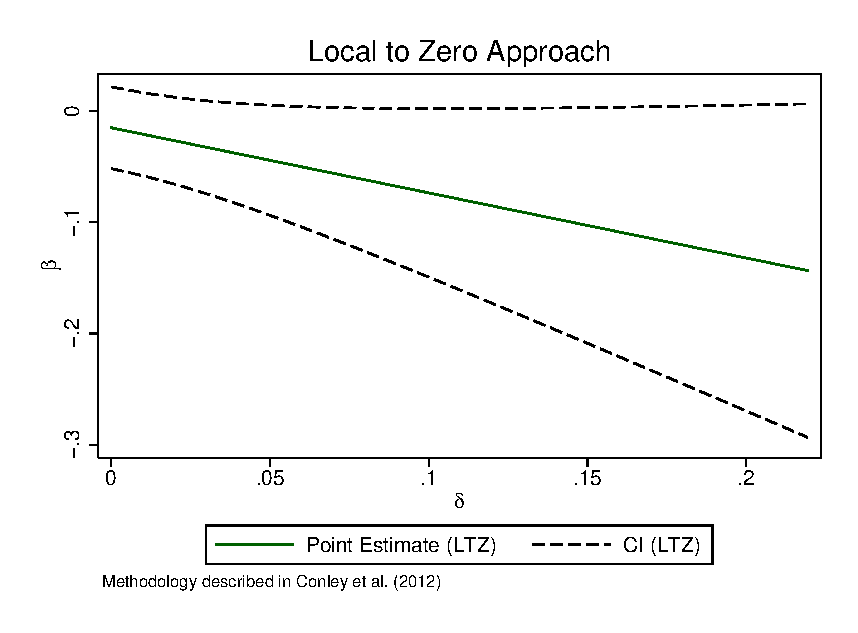
\includegraphics[scale=0.88]{\twinfolder/Figures/LTZ_two.eps}
\vspace{-8mm}
\floatfoot{Note to figure \ref{TWINfig:ltz2}: See note to Figure \ref{TWINfig:ltz3}}
\end{center}
\end{figure}

\begin{figure}[htpb!]
\begin{center}
\caption{Relaxing Strict Exogeneity (three plus)}
\label{TWINfig:ltz3}
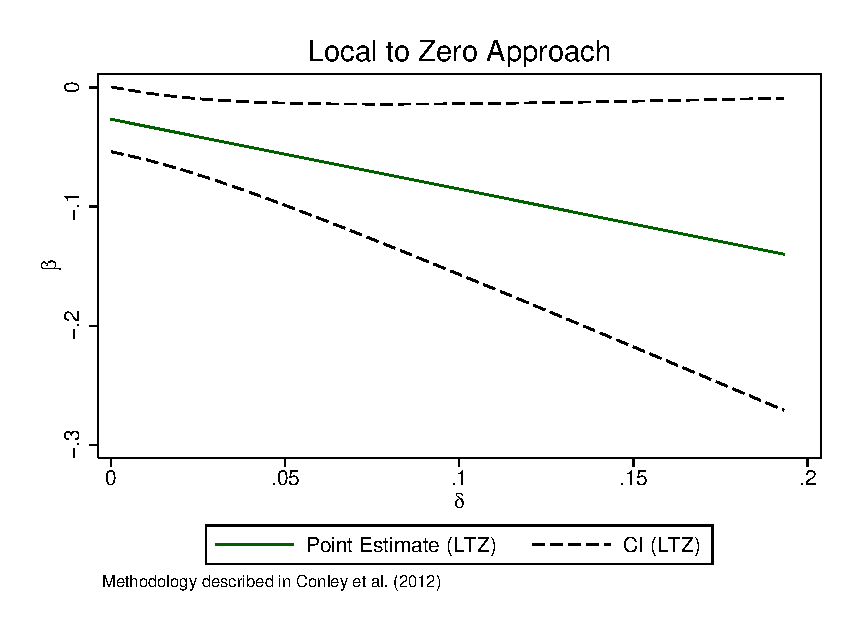
\includegraphics[scale=0.88]{\twinfolder/Figures/LTZ_three.eps} 
\floatfoot{Note to figure \ref{TWINfig:ltz3}: Confidence intervals and point estimates 
are calculated according to \citet{Conleyetal2012}.  Estimates reflect a range of priors 
regarding the validity of the exclusion restriction required to consistently estimate 
$\hat\beta_{fert}$ using twinning in a 2SLS framework.  The local to zero (LTZ) 
approach applied here assumes that $\gamma$, the sign on the instrument when included
in the first stage, is distributed $\gamma\sim U(0,\delta)$.  Further discussion 
is provided in the body of the text and table \ref{TWINtab:Conley}.}
\end{center}
\end{figure}

\begin{figure}[htpb!]
\begin{center}
\caption{Intra- and Inter-country trends: height and twinning}
\label{TWINfig:arrows}
\includegraphics[scale=0.86]{\twinfolder/Figures/height_country.eps} 
\end{center}
\end{figure}

